% Options for packages loaded elsewhere
\PassOptionsToPackage{unicode}{hyperref}
\PassOptionsToPackage{hyphens}{url}
%
\documentclass[
]{article}
\usepackage{amsmath,amssymb}
\usepackage{iftex}
\ifPDFTeX
  \usepackage[T1]{fontenc}
  \usepackage[utf8]{inputenc}
  \usepackage{textcomp} % provide euro and other symbols
\else % if luatex or xetex
  \usepackage{unicode-math} % this also loads fontspec
  \defaultfontfeatures{Scale=MatchLowercase}
  \defaultfontfeatures[\rmfamily]{Ligatures=TeX,Scale=1}
\fi
\usepackage{lmodern}
\ifPDFTeX\else
  % xetex/luatex font selection
\fi
% Use upquote if available, for straight quotes in verbatim environments
\IfFileExists{upquote.sty}{\usepackage{upquote}}{}
\IfFileExists{microtype.sty}{% use microtype if available
  \usepackage[]{microtype}
  \UseMicrotypeSet[protrusion]{basicmath} % disable protrusion for tt fonts
}{}
\makeatletter
\@ifundefined{KOMAClassName}{% if non-KOMA class
  \IfFileExists{parskip.sty}{%
    \usepackage{parskip}
  }{% else
    \setlength{\parindent}{0pt}
    \setlength{\parskip}{6pt plus 2pt minus 1pt}}
}{% if KOMA class
  \KOMAoptions{parskip=half}}
\makeatother
\usepackage{xcolor}
\usepackage[margin=1in]{geometry}
\usepackage{longtable,booktabs,array}
\usepackage{calc} % for calculating minipage widths
% Correct order of tables after \paragraph or \subparagraph
\usepackage{etoolbox}
\makeatletter
\patchcmd\longtable{\par}{\if@noskipsec\mbox{}\fi\par}{}{}
\makeatother
% Allow footnotes in longtable head/foot
\IfFileExists{footnotehyper.sty}{\usepackage{footnotehyper}}{\usepackage{footnote}}
\makesavenoteenv{longtable}
\usepackage{graphicx}
\makeatletter
\def\maxwidth{\ifdim\Gin@nat@width>\linewidth\linewidth\else\Gin@nat@width\fi}
\def\maxheight{\ifdim\Gin@nat@height>\textheight\textheight\else\Gin@nat@height\fi}
\makeatother
% Scale images if necessary, so that they will not overflow the page
% margins by default, and it is still possible to overwrite the defaults
% using explicit options in \includegraphics[width, height, ...]{}
\setkeys{Gin}{width=\maxwidth,height=\maxheight,keepaspectratio}
% Set default figure placement to htbp
\makeatletter
\def\fps@figure{htbp}
\makeatother
\setlength{\emergencystretch}{3em} % prevent overfull lines
\providecommand{\tightlist}{%
  \setlength{\itemsep}{0pt}\setlength{\parskip}{0pt}}
\setcounter{secnumdepth}{-\maxdimen} % remove section numbering
\usepackage{titlesec}
\titleformat{\section}{\centering\normalfont\Large\bfseries}{\thesection}{1em}{}
\titleformat{\subsection}{\centering\normalfont\large\bfseries}{\thesubsection}{1em}{}
\titleformat{\subsubsection}{\centering\normalfont\normalsize\bfseries}{\thesubsubsection}{1em}{}

\usepackage{silence}
\WarningsOff*
\usepackage{booktabs}
\usepackage{longtable}
\usepackage{array}
\usepackage{multirow}
\usepackage{wrapfig}
\usepackage{float}
\usepackage{colortbl}
\usepackage{pdflscape}
\usepackage{tabu}
\usepackage{threeparttable}
\usepackage{threeparttablex}
\usepackage[normalem]{ulem}
\usepackage{makecell}
\usepackage{xcolor}
\ifLuaTeX
  \usepackage{selnolig}  % disable illegal ligatures
\fi
\usepackage{bookmark}
\IfFileExists{xurl.sty}{\usepackage{xurl}}{} % add URL line breaks if available
\urlstyle{same}
\hypersetup{
  pdftitle={Análisis del nivel educativo de los padres y el tipo de alimentacion de los estudiantes como posibles indicadores del rendimiento academico de los mismos mediante metodos estadisticos},
  pdfauthor={David Mazza, Eros Bande, Sofia Rodriguez},
  hidelinks,
  pdfcreator={LaTeX via pandoc}}

\title{Análisis del nivel educativo de los padres y el tipo de
alimentacion de los estudiantes como posibles indicadores del
rendimiento academico de los mismos mediante metodos estadisticos}
\author{David Mazza, Eros Bande, Sofia Rodriguez}
\date{2025-03-10}

\begin{document}
\maketitle

\subsection{HIPOTESIS}\label{hipotesis}

La alimentación de los estudiantes y el nivel educativo de los padres
influye significativamente en el rendimiento académico de sus hijos, de
modo que, a mayor nivel educativo de los padres, mayor será el
rendimiento académico de los hijos.

\subsection{DESCRIPCION}\label{descripcion}

Esta investigación tiene como principal enfoque analizar como el nivel
educativo de los padres y la alimentación disponible para los
estudiantes se relaciona con los resultados de las calificaciones
obtenidas en tres exámenes distintos, tomando como base un grupo
representativo de colegiales estado unidenses con la finalidad de
presentar información concreta de los resultados obtenidos para que las
instituciones pertinentes diseñen planes de acción.

El rendimiento académico es uno de los pilares fundamentales del sistema
educativo, este no solo refleja las habilidades intelectuales
individuales de los alumnos, sino que también está influenciado por
factores externos, como el entorno familiar, el apoyo recibido y el
nivel educativo de los padres. Estudios previos han destacado el papel
de estas variables externas en la productividad académica de los
estudiantes.

En particular, el nivel educativo de los padres puede influir de
diversas maneras: fomentando una cultura de estudio, sirviendo como
modelo a seguir y brindando apoyo académico. Por otro lado, la
alimentación adecuada incide directamente en la capacidad de
concentración, un aspecto crucial para el éxito en cualquier ámbito
académico.

Aunque muchas personas podrían afirmar, por lógica o experiencia, que
estas variables influyen en el desempeño estudiantil, es fundamental
respaldar estas afirmaciones con indicadores y análisis estadísticos que
eliminen la subjetividad y las opiniones personales. Comprender esta
relación permitirá identificar áreas que requieren atención y diseñar
herramientas que favorezcan un entorno propicio para el rendimiento
académico.

\subsection{JUSTIFICACION}\label{justificacion}

El rendimiento académico de los estudiantes es un tema de gran
relevancia en el ámbito educativo, ya que está estrechamente vinculado a
oportunidades futuras y al desarrollo socioeconómico. Por ende,
identificar las variables que pueden predecir el rendimiento escolar es
de gran importancia para implementar soluciones efectivas, ya sea
mediante ayudas gubernamentales, campañas de concientización o programas
de apoyo específicos.

Diversos estudios han sugerido que el nivel educativo de los padres
puede ser un factor determinante en el éxito escolar de los hijos,
debido a la influencia que ejercen en la formación de hábitos de
estudio, la motivación y el acceso a recursos culturales, educativos y
alimenticios. Sin embargo, en el contexto local, existe una brecha en la
investigación que aborde esta relación de manera específica. Este
estudio busca contribuir a la comprensión de este fenómeno,
proporcionando información valiosa para diseñar políticas educativas y
estrategias que apoyen a las familias en la promoción del éxito
académico de sus hijos.

Un país con una educación sólida es sinónimo de progreso y desarrollo.
Para mejorar el sistema educativo, es necesario prestar atención a su
comportamiento de manera detallada y basada en información confiable, la
estadística se convierte así en la herramienta más efectiva para
lograrlo.

\subsection{OBJETIVOS}\label{objetivos}

\subsubsection{Objetivo general:}\label{objetivo-general}

\begin{itemize}
\tightlist
\item
  Analizar la relación entre el nivel educativo de los padres y la
  alimentación de los estudiantes con su desempeño académico en exámenes
  de habilidad verbal, matemática e inglés.
\end{itemize}

\subsubsection{Objetivos específicos:}\label{objetivos-especuxedficos}

\begin{itemize}
\item
  Realizar un análisis descriptivo de las variables nivel educativo de
  los padres, la alimentación de los estudiantes y las calificaciones de
  los estudiantes en los exámenes establecidos.
\item
  Establecer la relación entre el nivel educativo de los padres y los
  resultados de los estudiantes en los exámenes de habilidad verbal,
  matemática e inglés.
\item
  Determinar si la alimentación de los estudiantes está relacionada con
  el rendimiento académico en los exámenes mencionados.
\item
  Determinar cuál de las dos variables es más influyente en el desempeño
  escolar.
\end{itemize}

\subsection{VARIABLES}\label{variables}

\begin{itemize}
\tightlist
\item
  Nota en exámenes: Este es el principal indicador de desempeño
  académico y se expresa en los resultados de 3 distintas pruebas,
  matemáticas, lectura y escritura. Es una variable cuantitativa
  discreta
\item
  Nivel educativo de los padres: Es el nivel más alto de educación
  alcanzado por los responsables de los estudiantes. Este tendrá
  distintas categorías, como educación primaria, secundaria, superior,
  entre otros. Es una variable cualitativa ordinal. Esta variable consta
  de las categorías:

  \begin{itemize}
  \item
    Alguna educación secundaria: Indica que los padres no completaron la
    educación secundaria.
  \item
    Educación secundaria: Se refiere a que los padres completaron la
    escuela secundaria, incluyendo aquellos que lo hicieron a través de
    programas de equivalencia como el GED.
  \item
    Alguna educación universitaria: Se refiere a los padres que
    asistieron a la universidad, pero no obtuvieron un título. Esto
    puede incluir la obtención de créditos, diplomas o certificados.
  \item
    Título de asociado: Indica que los padres obtuvieron un título de
    asociado, que generalmente se obtiene en dos años en un colegio
    comunitario o escuela vocacional.
  \item
    Título de licenciatura o superior: Significa que los padres
    completaron un programa de licenciatura (cuatro años o más) o
    incluso un nivel de educación superior, como una maestría o un
    doctorado.
  \end{itemize}
\item
  Almuerzo de los estudiantes: Se considera la calidad del almuerzo de
  los estudiantes en dos categorías, estándar y sin almuerzo o reducido.
  Es una variable cualitativa nominal

  \begin{itemize}
  \tightlist
  \item
    Sin almuerzo o reducido: Alimentación deficiente en la que se
    presentan carencias de nutrientes importantes en el desarrollo de
    una persona de edad temprana, que tiene consecuencias cognitivas a
    largo plazo
  \item
    Estándar: Alimentación balanceada en la que se cumplen todas las
    necesidades básicas.
  \end{itemize}
\end{itemize}

Estas variables fueron seleccionadas porque representan factores
externos que, aunque no son elegidos por los estudiantes, tienen un gran
impacto en sus vidas. El nivel educativo de los padres y la alimentación
diaria son determinantes en las posibilidades académicas, recreativas y
alimenticias de un individuo, aspectos que, a su vez, pueden influir en
su rendimiento académico. Determinar si esto se cumple o no, será el
objetivo de esta investigación.

\subsection{LIMITES Y ALCANCE}\label{limites-y-alcance}

El límite de esta investigación recae en el alcance de la conclusión
establecida. Es decir, el enfoque principal del trabajo es establecer la
relación de las dos variables ya mencionadas con el desempeño
estudiantil, las razones específicas de el por qué esto sucede está más
allá del alcance de los datos disponibles.

\subsection{ANTECEDENTES}\label{antecedentes}

Un tema de gran interés global es el rendimiento escolar de los
estudiantes ya dado su relevancia en el crecimiento individual y, por
ende, su reflejo a nivel social. Existen diversos estudios que exploran
diferentes variables y como estos influyen en el desempeño escolar,
algunos de estos son el nivel educativo de los padres y la alimentación
de los estudiantes.

El nivel educativo de los padres puede influir de muchas maneras, un
artículo de la organización ClearingHouse (2020) realizó una síntesis de
estudios externos y determino que el comportamiento de los estudiantes
se moldea por la observación y experiencias formativas directas, es
decir, cuando los padres muestran un comportamiento orientado a logros
académicos, avance en carreras universitarias, postgrados,
investigaciones, y facilitan oportunidades de este tipo para sus hijos,
estos empiezan a creer en la importancia de este comportamiento y lo
priorizan.

Además, otro factor importante en el desempeño académico es la cantidad
de tiempo que pasan los estudiantes con sus padres, especialmente si es
de calidad y enfocado a desarrollar sus talentos. ClearingHouse (2020)
establece lo siguiente:

``Since children learn, in part, by observation, one of the key
components to a child's success is parental time investment (Kalil,
Ryan, \& Corey, 2012). Highly educated parents spend more time with
their children (Guryan, Hurst, \& Kearney, 2008) and spend that time
actively developing their children's talents and skills (Lareau, 2002)''

(Como los niños aprenden, en parte, por observación, uno de los
componentes claves para su éxito es la inversión de tiempo parental.
Padres altamente educados pasan más tiempo con sus hijos y enfocan ese
tiempo en desarrollar activamente sus talentos y habilidades. Traducción
propia)

Distintos estudios argumentan que el nivel educativo de los padres no
necesariamente tiene una relación directa con el desempeño estudiantil,
sin embargo, otros académicos concluyen que si tiene una influencia
notable en el tiempo que dedican a sus hijos y a su educación, a pesar
de que su tiempo podría ser enfocado en otras actividades laborales de
mayor remuneración.

``The level of parental education is correlated with the amount of time
spent with children and argue that more educated parents spend more time
with their children. For example, Guryan et al.~found that mothers with
a college education or higher spend more than 4 hours per week with
their children than mothers with lower education.'' Kantova, K. (2024)

(El nivel de educacion de los padres esta correlacionado con la cantidad
de tiempo invertido con sus hijos y argumenta que los padres más
educados pasan más tiempo con sus hijos. Por ejemplo, Guryan et al
encontró que las madres con una educación universitaria o mayor pasan
más de 4 horas por semana con sus hijos que las madres con menos
educación. Traducción propia)

Además, Kantova (2024) establece a través de numerosas citas y
referencias a otros académicos que el porcentaje de graduación de High
school (Preparatoria o bachillerato) es menor en individuos que
pertenencen a un nucleo familiar de bajo nivel educativo comparado a
aquellos de familias más educadas, específicamente, un 72\% a 87\%
respectivamente. Esto es sumamente preocupante a nivel económico y
social. Kantova (2024) establece:

``Belfield and Levin (2007) claim that high school graduation is a
doorway to economic self-sufficiency and civic engagement. Without a
high school diploma, people are more likely to earn a lower income and
be arrested, which leads to higher costs for the US.'' (Belfield y Levin
(2007) afirman que graduarse de preparatoria es una puerta a la
autosuficiencia económica y el compromiso cívico. Sin un diploma de
preparatoria, las personas son más propensas a tener un menor ingreso
económico y a ser arrestar, lo que causa mayor costo para Estados
Unidos. Traducción propia)

Por otra parte, la fundación Amhersth Wilder Foundation explica la
importancia de una buena alimentación en el desarrollo integral de los
niños, proceso social y académico. Se ha demostrado que una alimentación
pobre o reducida afecta la capacidad de pensamiento, conducta y salud,
factores que influencia el desempeño estudiantil (Wilder Research, 2014)

Se han realizado numerosos estudios sobre este tema, prohibir comida
chatarra en campañas escolares y ofrecer alternativas más saludables en
las comidas. Esta investigación encontró que los estudiantes de las
escuelas donde se implementó esta idea tuvieron mejores calificaciones
en algunas materias comparado a quienes no estuvieron involucrados en el
experimento (Belot \& Jamesm 2009, como se citó en Wilder research,
2014)

Una nutrición balanceada, que satisfaga todas las necesidades
alimenticias de los estudiantes no solo evita enfermedades que afecten
la asistencia y desempeño escolar, también les da más energías a los
estudiantes, aumenta su concentración e incluso promueve su capacidad
cognitiva. (Bellisle, 2004; Sorhaindo \& Feinstein, 2006, como se citó
en Wilder research, 2014)

Malki, A (2018) realizó un estudio titulado ``Effects of Student
Nutrition on Academic Perfomance'' (Efectos de la nutrición escolar en
el desempeño academico) y determinó que los estudiantes que tenían una
situación de inseguridad alimenticia tenían una tendencia a un desempeño
escolar menor comparado con los demás, aquellos que consumían 2 comidas
por día tenían una tendencia a un rendimiento medio y los que tenían
acceso a comidas saludables y balanceadas, en promedio, tenían mejor
rendimiento. Esto fue determinado a través de un análisis de regresión
lineal.

A continuación, se mostraran los calculos descriptivos de la variable
cuantitativa llamada Desempeño, esta es sera utilizada como la sintesis
del desempeño escolar de los estudiantes

\begin{longtable}[]{@{}
  >{\centering\arraybackslash}p{(\columnwidth - 16\tabcolsep) * \real{0.1176}}
  >{\centering\arraybackslash}p{(\columnwidth - 16\tabcolsep) * \real{0.1059}}
  >{\centering\arraybackslash}p{(\columnwidth - 16\tabcolsep) * \real{0.1176}}
  >{\centering\arraybackslash}p{(\columnwidth - 16\tabcolsep) * \real{0.1412}}
  >{\centering\arraybackslash}p{(\columnwidth - 16\tabcolsep) * \real{0.0941}}
  >{\centering\arraybackslash}p{(\columnwidth - 16\tabcolsep) * \real{0.1176}}
  >{\centering\arraybackslash}p{(\columnwidth - 16\tabcolsep) * \real{0.1176}}
  >{\centering\arraybackslash}p{(\columnwidth - 16\tabcolsep) * \real{0.0941}}
  >{\centering\arraybackslash}p{(\columnwidth - 16\tabcolsep) * \real{0.0941}}@{}}
\caption{Cálculo de medidas descriptivas}\tabularnewline
\toprule\noalign{}
\begin{minipage}[b]{\linewidth}\centering
Promedio
\end{minipage} & \begin{minipage}[b]{\linewidth}\centering
Mediana
\end{minipage} & \begin{minipage}[b]{\linewidth}\centering
Varianza
\end{minipage} & \begin{minipage}[b]{\linewidth}\centering
D.Estandar
\end{minipage} & \begin{minipage}[b]{\linewidth}\centering
CV
\end{minipage} & \begin{minipage}[b]{\linewidth}\centering
Kurtosis
\end{minipage} & \begin{minipage}[b]{\linewidth}\centering
Simetria
\end{minipage} & \begin{minipage}[b]{\linewidth}\centering
Minimo
\end{minipage} & \begin{minipage}[b]{\linewidth}\centering
Maximo
\end{minipage} \\
\midrule\noalign{}
\endfirsthead
\toprule\noalign{}
\begin{minipage}[b]{\linewidth}\centering
Promedio
\end{minipage} & \begin{minipage}[b]{\linewidth}\centering
Mediana
\end{minipage} & \begin{minipage}[b]{\linewidth}\centering
Varianza
\end{minipage} & \begin{minipage}[b]{\linewidth}\centering
D.Estandar
\end{minipage} & \begin{minipage}[b]{\linewidth}\centering
CV
\end{minipage} & \begin{minipage}[b]{\linewidth}\centering
Kurtosis
\end{minipage} & \begin{minipage}[b]{\linewidth}\centering
Simetria
\end{minipage} & \begin{minipage}[b]{\linewidth}\centering
Minimo
\end{minipage} & \begin{minipage}[b]{\linewidth}\centering
Maximo
\end{minipage} \\
\midrule\noalign{}
\endhead
\bottomrule\noalign{}
\endlastfoot
67.77 & 68.33 & 203.27 & 14.26 & 21.04\% & 0.11 & -0.3 & 9 & 100 \\
\end{longtable}

\begin{center}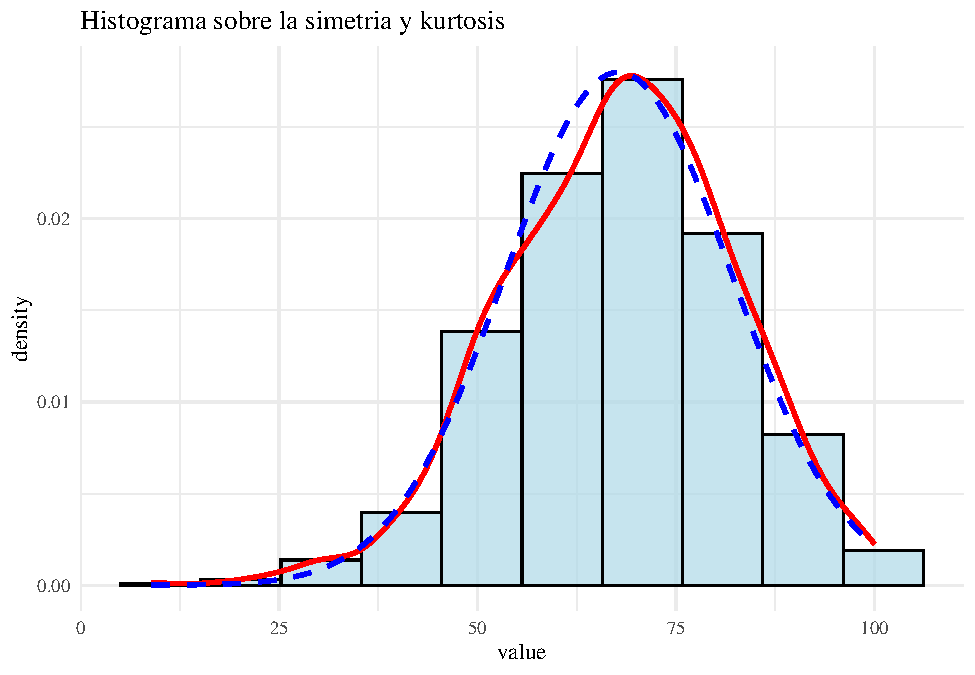
\includegraphics{Trabajo-Grupo-6.-Students-performance_files/figure-latex/unnamed-chunk-1-1} \end{center}

Estas son las distribuciones de las variables cualitativas, en cantidad
total, proporcion y graficos que faciliten su comprensión

\begin{longtable}[]{@{}ccc@{}}
\caption{Distribución de la variable parental level of
education}\tabularnewline
\toprule\noalign{}
parental level of education & Cantidad1 & Proporcion1 \\
\midrule\noalign{}
\endfirsthead
\toprule\noalign{}
parental level of education & Cantidad1 & Proporcion1 \\
\midrule\noalign{}
\endhead
\bottomrule\noalign{}
\endlastfoot
associate's degree & 222 & 22.2 \\
bachelor's degree & 118 & 11.8 \\
high school & 196 & 19.6 \\
master's degree & 59 & 5.9 \\
some college & 226 & 22.6 \\
some high school & 179 & 17.9 \\
\end{longtable}

\begin{longtable}[]{@{}ccc@{}}
\caption{Distribución de la variable lunch}\tabularnewline
\toprule\noalign{}
lunch & Cantidad2 & Proporcion2 \\
\midrule\noalign{}
\endfirsthead
\toprule\noalign{}
lunch & Cantidad2 & Proporcion2 \\
\midrule\noalign{}
\endhead
\bottomrule\noalign{}
\endlastfoot
free/reduced & 355 & 35.5 \\
standard & 645 & 64.5 \\
\end{longtable}

\begin{center}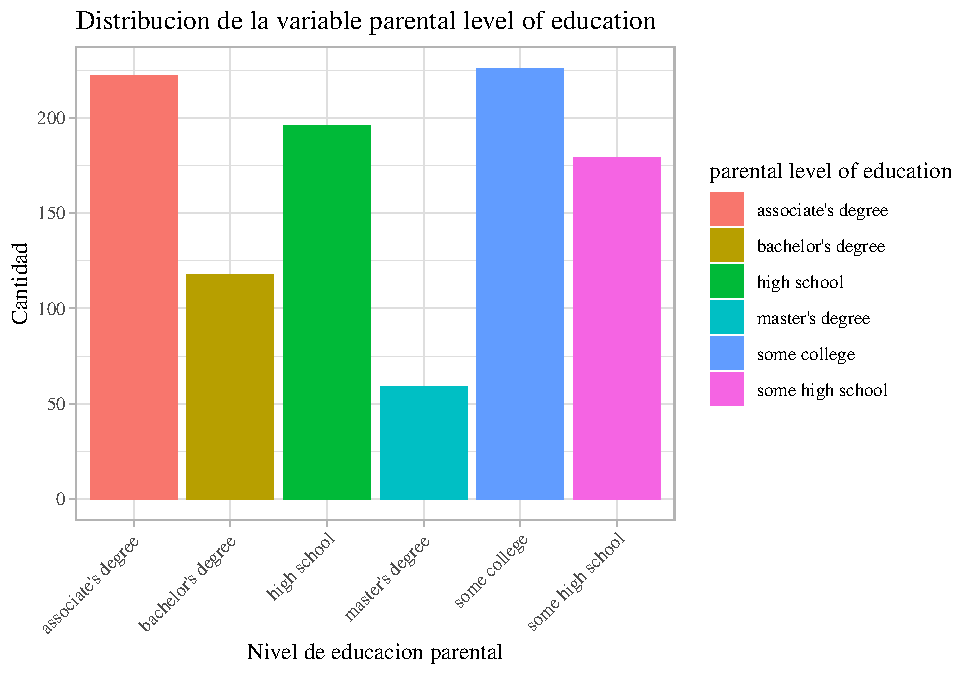
\includegraphics{Trabajo-Grupo-6.-Students-performance_files/figure-latex/unnamed-chunk-2-1} \end{center}

\begin{center}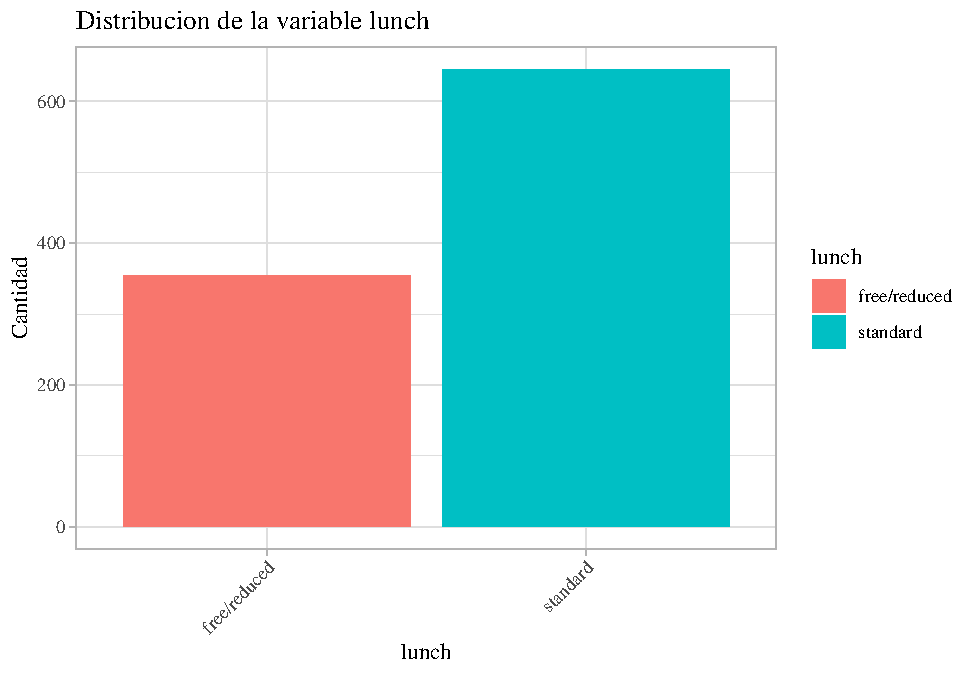
\includegraphics{Trabajo-Grupo-6.-Students-performance_files/figure-latex/unnamed-chunk-2-2} \end{center}

\begin{center}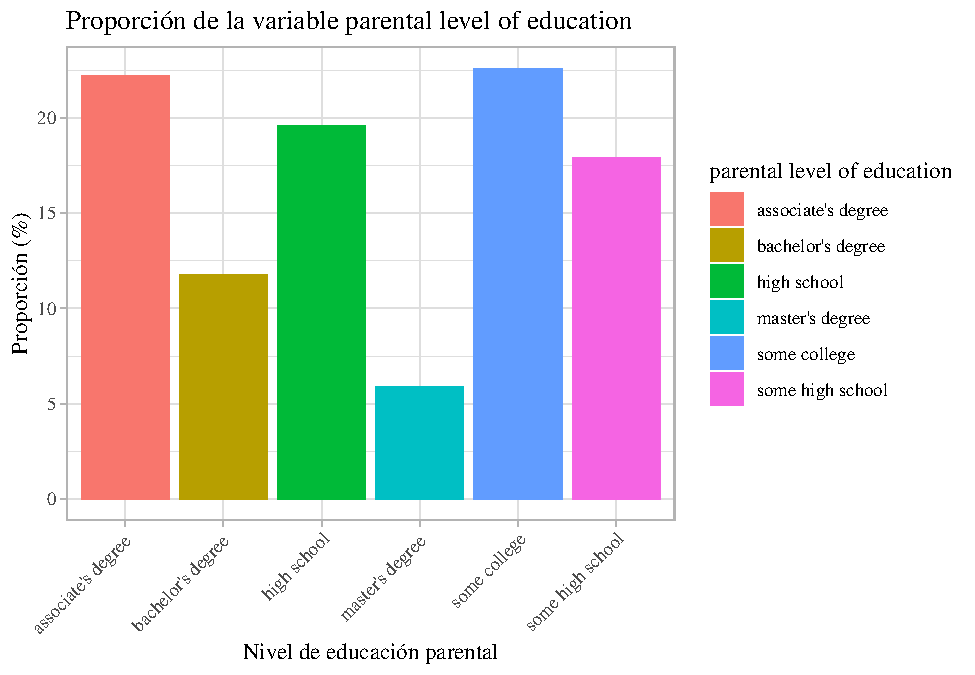
\includegraphics{Trabajo-Grupo-6.-Students-performance_files/figure-latex/unnamed-chunk-2-3} \end{center}

\begin{center}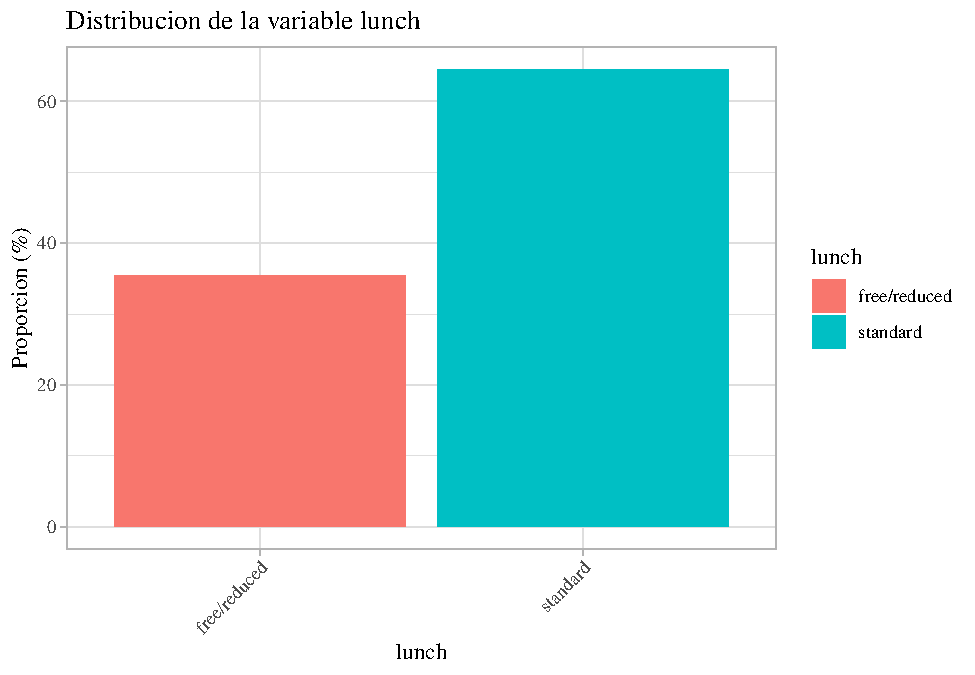
\includegraphics{Trabajo-Grupo-6.-Students-performance_files/figure-latex/unnamed-chunk-2-4} \end{center}

\section{Analisis Bivariante}\label{analisis-bivariante}

Para examinar si existe alguna clase de correlación entre las variables
``Nivel Educativo de los padres'' y ``Almuerzo'' en comparación a la
variable ``Desempeño'' analisaremos las proporciones, los cuartiles y la
asimetria y kurtosis de desempeño en relacion a las otras variables.

\begin{table}[!h]
\centering
\caption{\label{tab:tabla de frecuencias relativas porcentuales 1 }Frecuencias Relativas del Desempeño en Comparación al Nivel Educativo de los Padres}
\centering
\begin{tabular}[t]{lrrrrr}
\toprule
  & {}[9,32] & {}[32,55] & {}[55,78] & {}[78,100] & Sum\\
\midrule
\cellcolor{gray!10}{associate's degree} & \cellcolor{gray!10}{0.23} & \cellcolor{gray!10}{8.33} & \cellcolor{gray!10}{27.25} & \cellcolor{gray!10}{14.19} & \cellcolor{gray!10}{50}\\
bachelor's degree & 0.00 & 5.08 & 28.81 & 16.10 & 50\\
\cellcolor{gray!10}{high school} & \cellcolor{gray!10}{1.02} & \cellcolor{gray!10}{13.52} & \cellcolor{gray!10}{28.32} & \cellcolor{gray!10}{7.14} & \cellcolor{gray!10}{50}\\
master's degree & 0.00 & 5.93 & 23.73 & 20.34 & 50\\
\cellcolor{gray!10}{some college} & \cellcolor{gray!10}{0.88} & \cellcolor{gray!10}{6.42} & \cellcolor{gray!10}{29.87} & \cellcolor{gray!10}{12.83} & \cellcolor{gray!10}{50}\\
\addlinespace
some high school & 1.40 & 10.89 & 27.09 & 10.61 & 50\\
\cellcolor{gray!10}{Sum} & \cellcolor{gray!10}{0.70} & \cellcolor{gray!10}{8.85} & \cellcolor{gray!10}{28.00} & \cellcolor{gray!10}{12.45} & \cellcolor{gray!10}{50}\\
\bottomrule
\end{tabular}
\end{table}

En la tabla 1 se observa que los estudiantes cuyos padres tienen un
nivel educativo más alto (como ``bachelor's degree'' y ``master's
degree'') tienden a tener (en proporción) un mayor número de estudiantes
en los intervalos de desempeño más altos ({[}78,100{]}), por ejemplo, en
el intervalo {[}78,100{]}, los estudiantes con padres que tienen un
``master's degree'' tienen 24 estudiantes, mientras que los estudiantes
con padres que tienen un ``high school'' tienen solo 28 estudiantes, a
pesar de que el grupo de ``high school'' es mucho más grande (196
estudiantes en total) que el grupo de ``master's degree'' (con 59
estudiantes en total). Sin embargo busquemos visualizar esto de mejor
manera mediante cualtiles.

\begin{longtable}[t]{lrrr}
\caption{\label{tab:cuartiles}Cuartiles del Desempeño por Nivel Educativo de los Padres}\\
\toprule
parental level of education & Q1 & Q2 & Q3\\
\midrule
\cellcolor{gray!10}{associate's degree} & \cellcolor{gray!10}{58.67} & \cellcolor{gray!10}{69.67} & \cellcolor{gray!10}{79.00}\\
bachelor's degree & 64.08 & 71.16 & 80.67\\
\cellcolor{gray!10}{high school} & \cellcolor{gray!10}{53.92} & \cellcolor{gray!10}{65.00} & \cellcolor{gray!10}{72.67}\\
master's degree & 63.16 & 73.33 & 85.50\\
\cellcolor{gray!10}{some college} & \cellcolor{gray!10}{60.00} & \cellcolor{gray!10}{68.67} & \cellcolor{gray!10}{78.00}\\
\addlinespace
some high school & 55.66 & 66.67 & 76.50\\
\bottomrule
\end{longtable}

En la tabla 2 se observa que los estudiantes cuyos padres tienen un
nivel educativo más alto (como ``bachelor's degree'' y ``master's
degree'') tienen cuartiles más altos en comparación con aquellos cuyos
padres tienen un nivel educativo más bajo (como ``high school'' y ``some
high school''), por ejemplo, el Q3 (tercer cuartil) para ``master's
degree'' es 85.50, mientras que para ``high school'' es 72.67. Esto
indica que el 75\% de los estudiantes con padres que tienen un
``master's degree'' tienen un desempeño superior a 85.50, mientras que
el 75\% de los estudiantes con padres que tienen un ``high school''
tienen un desempeño superior a 72.67.Todo esto se puede visualizar mucho
mejor en el grafico de cajas ``Desempeño en función del Nivel Educativo
de los Padres''.

\begin{center}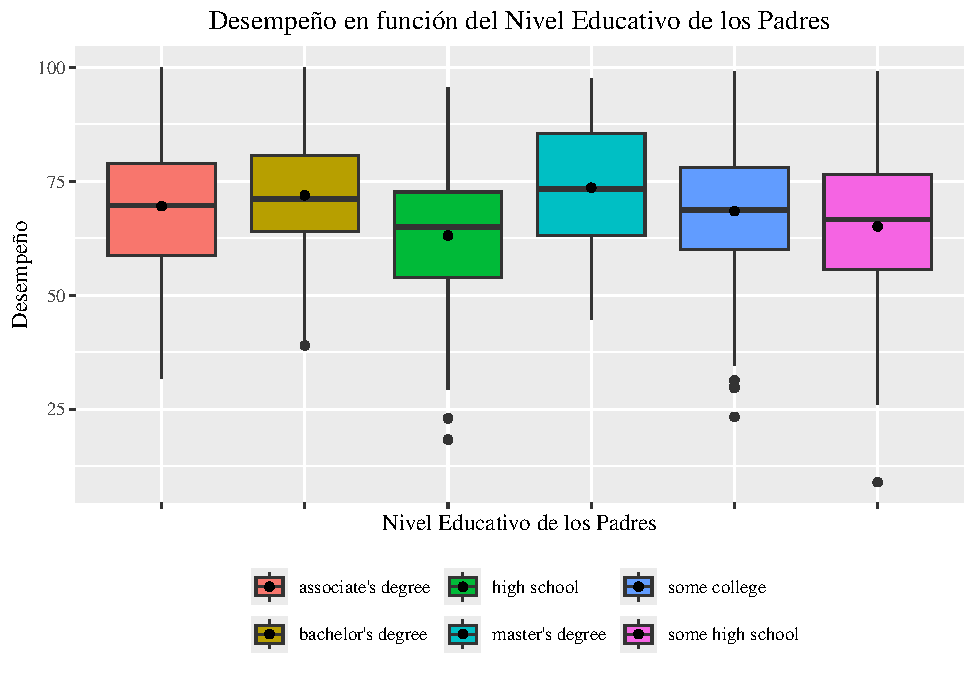
\includegraphics{Trabajo-Grupo-6.-Students-performance_files/figure-latex/grafico1-1} \end{center}

\begin{table}[!h]
\centering
\caption{\label{tab:caculos basicos}Estadisticas Basicas del Desempeño por Nivel Educativo de los Padres}
\centering
\begin{tabular}[t]{lrrrrr}
\toprule
parental level of education & Promedio & D.Estandar & CV & Asimetria & Kurtosis\\
\midrule
\cellcolor{gray!10}{associate's degree} & \cellcolor{gray!10}{69.57} & \cellcolor{gray!10}{13.67} & \cellcolor{gray!10}{19.65} & \cellcolor{gray!10}{-0.10} & \cellcolor{gray!10}{-0.65}\\
bachelor's degree & 71.92 & 13.95 & 19.40 & -0.03 & -0.34\\
\cellcolor{gray!10}{high school} & \cellcolor{gray!10}{63.10} & \cellcolor{gray!10}{13.51} & \cellcolor{gray!10}{21.41} & \cellcolor{gray!10}{-0.39} & \cellcolor{gray!10}{0.16}\\
master's degree & 73.60 & 13.60 & 18.48 & -0.12 & -0.99\\
\cellcolor{gray!10}{some college} & \cellcolor{gray!10}{68.48} & \cellcolor{gray!10}{13.71} & \cellcolor{gray!10}{20.02} & \cellcolor{gray!10}{-0.38} & \cellcolor{gray!10}{0.23}\\
\addlinespace
some high school & 65.11 & 14.98 & 23.01 & -0.56 & 0.38\\
\bottomrule
\end{tabular}
\end{table}

De la tabla 3 podemos notar que mientras mayor es el ``Nivel Educativo
de los Padres'' mayor es la media de ``Desempeño'' de de los
estudiantes, por ejemplo, ``master's degree'' tiene 73.6 puntos en
promedio por estudiante y ``bachelor's degree'' tiene 71.92 puntos en
promedio por estudiante, mientras que ``some high school'' tiene 65.11
puntos en promedio por estudiante y ``high school'' tiene 63.10 puntos
en promedio por estudiante. El coeficiente de variación es más bajo para
los niveles educativos más altos, lo que indica que el desempeño es más
consistente en estos grupos, por ejemplo, ``master's degree'' tiene un
18.48\% de variación de notas por estudiante y ``bachelor's degree''
tiene un 19.4\% de variación de notas por estudiante, mientras que
``some high school'' tiene un 23.01\% de variación de notas por
estudiante y ``high school'' tiene un 21.41\% de variación de notas por
estudiante. Y la asimetría y la curtosis muestran.

\begin{table}[!h]
\centering
\caption{\label{tab:tabla2 }Desempeño En Comparación al Tipo de Almuerzo}
\centering
\begin{tabular}[t]{lrrrrr}
\toprule
  & {}[9,32] & {}[32,55] & {}[55,78] & {}[78,100] & Sum\\
\midrule
\cellcolor{gray!10}{free/reduced} & \cellcolor{gray!10}{11} & \cellcolor{gray!10}{96} & \cellcolor{gray!10}{196} & \cellcolor{gray!10}{52} & \cellcolor{gray!10}{355}\\
standard & 3 & 81 & 364 & 197 & 645\\
\cellcolor{gray!10}{Sum} & \cellcolor{gray!10}{14} & \cellcolor{gray!10}{177} & \cellcolor{gray!10}{560} & \cellcolor{gray!10}{249} & \cellcolor{gray!10}{1000}\\
\bottomrule
\end{tabular}
\end{table}

En la tabla 4 podemos observar que los estudiantes que reciben un
almuerzo ``standard'' tienen un mayor número de estudiantes en los
intervalos de desempeño más altos en proporción que los que reciben un
almuerzo ``free/reduced'', por ejemplo, en el intervalo {[}78,100{]},
hay 197 estudiantes con almuerzo ``standard'' y solo 52 con almuerzo
``free/reduced'', esto sugiere que la calidad del almuerzo está
relacionada con un mejor rendimiento académico, pasemos a nalizar mejor
esto mediante cuartiles.

\begin{table}[!h]
\centering
\caption{\label{tab:cuartiles2}Cuartiles del Desempeño Calidad de Almuerzo}
\centering
\begin{tabular}[t]{lrrr}
\toprule
lunch & Q1 & Q2 & Q3\\
\midrule
\cellcolor{gray!10}{free/reduced} & \cellcolor{gray!10}{52.84} & \cellcolor{gray!10}{62.67} & \cellcolor{gray!10}{72.50}\\
standard & 62.33 & 71.33 & 79.67\\
\bottomrule
\end{tabular}
\end{table}

La tabla 5 muestra que los estudiantes que reciben un almuerzo
``standard'' tienen un desempeño más alto en comparación con los que
reciben un almuerzo ``free/reduced'', ya que los estudiantes con
almuerzo estandar tienen un ``Desempeño'' superior al de los estudiantes
con almuerzos ``free/reduced'', por ejemplo, el Q3 (tercer cuartil) para
``standard'' es de 79.67 puntos, mientras que para ``free/reduced'' es
de 72.50 puntos, esto indica que el 75\% de los estudiantes con almuerzo
``standard'' tienen un desempeño superior a 79.67 puntos, mientras que
el 75\% de los estudiantes con almuerzo ``free/reduced'' tienen un
desempeño superior a 72.50 puntos, todo esto se puede observar mucho
mejor en el grafico ``Desempeño en función de la Calidad de los
Almuerzos''.

\begin{center}\includegraphics{Trabajo-Grupo-6.-Students-performance_files/figure-latex/grafico2-1} \end{center}

\begin{table}[!h]
\centering
\caption{\label{tab:calculos basicos2}Estadisticas Basicas del Desempeño por Calidad de Almuerzo}
\centering
\begin{tabular}[t]{lrrrrr}
\toprule
lunch & Promedio & D.Estandar & CV & Asimetria & Kurtosis\\
\midrule
\cellcolor{gray!10}{free/reduced} & \cellcolor{gray!10}{62.20} & \cellcolor{gray!10}{14.46} & \cellcolor{gray!10}{23.25} & \cellcolor{gray!10}{-0.31} & \cellcolor{gray!10}{0.22}\\
standard & 70.84 & 13.19 & 18.62 & -0.19 & -0.19\\
\bottomrule
\end{tabular}
\end{table}

\section{Comparación de las Tres Variables en
Conjunto}\label{comparaciuxf3n-de-las-tres-variables-en-conjunto}

\begin{center}\includegraphics{Trabajo-Grupo-6.-Students-performance_files/figure-latex/grafico3-1} \end{center}

\end{document}
